\documentclass[conference]{IEEEtran}
\usepackage{cite}
\usepackage{amsmath,amssymb,amsfonts}
\usepackage{algorithmic}
\usepackage{graphicx}
\graphicspath{{./}{Figures/}{./Figures/}}
\usepackage{textcomp}
\usepackage{xcolor}
\usepackage{hyperref}
\usepackage{listings}
\usepackage{array}
\renewcommand{\arraystretch}{1.2}
\makeatletter
\newcommand{\linebreakand}{%
  \end{@IEEEauthorhalign}
  \hfill\mbox{}\par
  \mbox{}\hfill\begin{@IEEEauthorhalign}
}
\makeatother
\begin{document}

\title{AI-Based Automated Log Analysis and Performance Evaluation System for Emulation-Based Pre-Silicon Software Testing}

\author{
    \IEEEauthorblockN{Vijay Kumar Prajapati}
    \IEEEauthorblockA{\textit{Dept. of ECE} \\
    \textit{RV College of Engineering}\\
    Bangalore, India \\
    vijaykumarp.ec22@rvce.edu.in}
    \and
    \IEEEauthorblockN{Dr. Roopa J}
    \IEEEauthorblockA{\textit{Dept. of ECE} \\
    \textit{RV College of Engineering}\\
    Bangalore, India \\
    roopaj@rvce.edu.in}
    \and
    \IEEEauthorblockN{Venkatarakesh Mamidi}
    \IEEEauthorblockA{\textit{Emulation \& Pre-Silicon Validation} \\
    \textit{Qualcomm India Pvt. Ltd.}\\
    Bangalore, India \\
    vmamidi@qti.qualcomm.com}
}

\maketitle

\begin{abstract}
The pre-silicon validation of modern System-on-Chip (SoC) designs depends critically on the ability to interpret a large volume of emulation logs that are produced for each regression run. Manual analysis of these logs is repetitive, error-prone and consumes a significant fraction of an engineer's working day. This paper presents an AI-based automated log analysis and performance evaluation system that integrates LogPAI's Drain algorithm for structured log parsing, the LogAI framework for unsupervised clustering and anomaly detection, regular-expression-driven metric extraction, and a Large Language Model (LLM) based stage for natural-language summary generation and root-cause direction. The proposed pipeline is implemented in Python 3 on a Linux-based emulation platform and is validated on a fixed test suite of twelve representative graphs across six silicon configurations - one Cascade baseline and five Nova variants. Experimental results show that the pipeline reduces regression analysis time from several hours of manual work to approximately two minutes per regression. On the test suite, the system correctly identifies that Nova-Alpha (787\,MHz) exhibits seven degraded tests, while Nova-Delta and Nova-Epsilon (1037\,MHz) exhibit only one each. A detailed root-cause analysis of MosaicNet\_W8A8 isolates Coproc\_2 stalls as the dominant bottleneck, with a stall percentage difference of $-113\%$ relative to the baseline. The combination of structured parsing, machine learning and LLM-based reasoning enables both fast degradation detection and actionable root-cause hints, demonstrating the practical value of hybrid AI pipelines for industrial-scale pre-silicon validation.
\end{abstract}

\begin{IEEEkeywords}
Pre-silicon Validation, Log Analysis, Drain Algorithm, LogPAI, LogAI, Large Language Models, Performance Regression, System-on-Chip
\end{IEEEkeywords}

\section{Introduction}

The development of modern System-on-Chip (SoC) designs follows a hardware-software co-design methodology in which functional and performance targets must be met before silicon fabrication. Emulation platforms have therefore become indispensable to the pre-silicon validation flow, since they enable software test cases to be run against pre-RTL hardware models and capture detailed performance counters in the form of log files \cite{lai2018emulation, deltombe2014emulation}. For each regression run, the platform produces hundreds of log files containing throughput counters, memory bandwidth, stall cycles, and a broad range of microarchitectural state. The size and complexity of these logs has grown rapidly with the size of the silicon under test, and engineers in the validation team often spend a significant fraction of their working day on extracting, transcribing and comparing these counters across configurations \cite{he2021survey}.

The traditional manual workflow consists of (i) navigating to the log directory of the option under test, (ii) using \texttt{grep} to find cycles, instructions per second (IPS), bandwidth and stall counters, (iii) copying the values into a spreadsheet, (iv) computing percentage differences against a baseline configuration, and (v) writing a short summary for the engineering team. On a typical regression with twelve graphs across six options, this manual workflow can take between one and a half and three hours per regression and is prone to transcription errors and naming inconsistencies between engineers. As validation timelines tighten and the number of silicon configurations under evaluation grows, this manual flow has become a bottleneck rather than a tool.

Recent advances in automated log parsing \cite{he2017drain, zhu2019tools, du2016spell}, log-based anomaly detection \cite{du2017deeplog, zhang2019logrobust, guo2021logbert}, and Large Language Model (LLM) based reasoning over log data \cite{le2023logprompt, liu2024logprompt, ahmed2023recommending} suggest a path towards a fully automated pipeline that replaces manual grepping with reproducible, AI-assisted analysis. However, most existing systems address only one stage of the workflow - parsing, detection, or summarization - and few attempts have been made to integrate the three stages into a single pipeline targeted at industrial pre-silicon validation.

\subsection{Problem Statement}
The fundamental challenge addressed in this work is to overcome the slow and error-prone manual analysis of extensive log data generated from large-scale emulation tests, and to effectively identify performance issues and direct engineers to their root cause. An automated system is required for efficient log extraction, analysis and summarization that improves debugging and decision-making across the validation team. The system must produce reproducible outputs that can be regenerated by any engineer, must compress regression analysis time from hours to minutes, and must surface degradations together with directional root-cause hints.

\subsection{Contributions}
This paper makes the following key contributions:
\begin{itemize}
\item \textbf{Hybrid AI Pipeline:} A four-stage pipeline that integrates LogPAI's Drain algorithm for structured log parsing, LogAI for ML-based clustering and anomaly detection, regular expressions for deterministic counter extraction, and an LLM API for summary generation and root-cause hints, all under one execution context.
\item \textbf{Degradation Detection Rules:} A combined rule set that flags a test as degraded only when both the throughput percentage difference and the dominant stall counter cross configurable thresholds, suppressing false positives caused by run-to-run variance.
\item \textbf{Quantitative Validation:} An empirical study on a fixed test suite of twelve graphs across six silicon configurations (one Cascade baseline and five Nova variants), with detailed per-graph IPS comparisons and a worked root-cause analysis of MosaicNet\_W8A8.
\item \textbf{Productivity Gains:} A reduction in per-regression analysis time from approximately one and a half to three hours of manual work down to about two minutes of pipeline execution, with deterministic and reproducible workbook outputs.
\item \textbf{Open Reference Implementation:} A modular Python 3 reference implementation organized as a set of cooperating modules (\texttt{ingest}, \texttt{preprocess}, \texttt{parse}, \texttt{extract}, \texttt{analyze}, \texttt{compare}, \texttt{report}, \texttt{llm}, \texttt{notify}).
\end{itemize}

\subsection{Paper Organization}
The remainder of this paper is organized as follows. Section II reviews related work in log parsing, anomaly detection, and LLM-based log understanding. Section III presents the proposed methodology, including the four-stage pipeline and the computational formulae. Section IV describes the experimental setup, including the test suite, the silicon configurations, and the evaluation methodology. Section V presents the results and analysis, including the degradation summary, the architectural effect on IPS, and the root-cause analysis. Section VI discusses the implications and limitations of the proposed approach. Section VII concludes with future directions.

\section{Related Work}

\subsection{Log Parsing Approaches}
Log parsing is the task of converting unstructured raw log lines into structured templates with separated constant and variable parts. Early approaches relied on hand-crafted regular expressions specific to each application, which are difficult to maintain at scale. Du et al. proposed Spell \cite{du2016spell}, which performs online streaming parsing using the longest common subsequence between log messages. He et al. introduced Drain \cite{he2017drain}, which builds a fixed-depth parse tree and walks tokens to a leaf to assign each line to a template; Drain has become a de facto standard because of its low computational complexity and competitive accuracy on the LogPAI benchmark suite \cite{zhu2019tools}.

More recently, LLM-based parsers have emerged. Le and Zhang's LogPrompt \cite{le2023logprompt} explores prompt-based few-shot learning for log parsing, while Zhang et al. introduce SemanticLog \cite{zhang2025semanticlog}, which improves accuracy and efficiency for large-scale semantic log parsing. Chen et al.'s EPAS \cite{chen2025epas} demonstrates that asynchronous scheduling of parsing tasks can substantially improve the throughput of online log parsers, which is directly applicable to industrial regression flows.

\subsection{Anomaly Detection in System Logs}
Once logs are parsed, anomaly detection identifies behaviour that deviates from a learned norm. Du et al. proposed DeepLog \cite{du2017deeplog}, which models the sequence of log keys as a stochastic process using LSTM networks and flags deviations as anomalies. Zhang et al.'s LogRobust \cite{zhang2019logrobust} addresses the problem of unstable log formats across software versions through attention-based bidirectional LSTMs and semantic vectorization. Guo et al.'s LogBERT \cite{guo2021logbert} uses self-supervised pretraining over masked log key sequences and demonstrates strong performance on the HDFS, BGL and Thunderbird datasets. The Salesforce LogAI library \cite{cheng2023logai} packages classical clustering, isolation-forest based anomaly detection and deep models behind a unified API; the present work uses LogAI as the basis of its analysis stage.

Wang et al. \cite{wang2025logdlr} extend the unsupervised setting with domain-invariant latent representations that improve cross-system anomaly detection on logs with very different formats, addressing the practical reality that emulation platforms generate logs from several heterogeneous sub-systems.

\subsection{LLM-Based Log Understanding}
Large Language Models such as GPT-style architectures \cite{vaswani2017attention, brown2020gpt3} have begun to play a central role in software engineering tasks, including log understanding. Liu et al.'s LUK framework \cite{liu2025luk} shows that incorporating LLM-derived expert knowledge significantly improves downstream log analysis. Ahmed et al.'s recommending-log-statements work \cite{ahmed2023recommending} demonstrates that LLMs can recommend appropriate log placement and verbosity, while Liu et al.'s LogPrompt \cite{liu2024logprompt} explores zero-shot and interpretable analysis. The present work builds on this line by using an LLM purely as a downstream summarization and root-cause-hint stage, while keeping the heavy lifting on deterministic parsers and ML clusterers.

\subsection{Performance Regression Analysis in Pre-Silicon Validation}
Pre-silicon performance validation has historically relied on hand-written cycle accounting and spreadsheet-based regression comparison \cite{lai2018emulation, deltombe2014emulation}. Industrial reports such as Li et al. \cite{li2025practitioners} highlight a persistent gap between academic anomaly detection research and the practical needs of validation teams: practitioners value interpretable, actionable summaries and reproducible reports more than raw model accuracy. The pipeline proposed in this paper is designed explicitly to close that gap by producing standardized three-sheet workbooks per regression and a multi-option comparison workbook per silicon variant.

\section{Methodology}

The proposed pipeline operates in four sequential stages: data collection, log processing, analysis engine, and output \& delivery. Each stage produces a well-defined artifact that gates the next stage, allowing the pipeline to be re-run from any intermediate point.

\subsection{Stage 1 - Data Collection}
The data collection stage executes software test cases on the emulation platform, ingests the raw log files, and stores them in a structured directory tree of the form \texttt{<regression\_id> / <option> / <graph>.log}. Once all logs are present, the stage signals \textit{Log Data Ready} for the next stage. The ingestion module also writes a small manifest that records the timestamp, build identifier, and random seed for each log so that any regression can be reproduced bit-exactly later. Figure \ref{fig:datacoll} illustrates the data collection flow.

\begin{figure}[t]
\centering
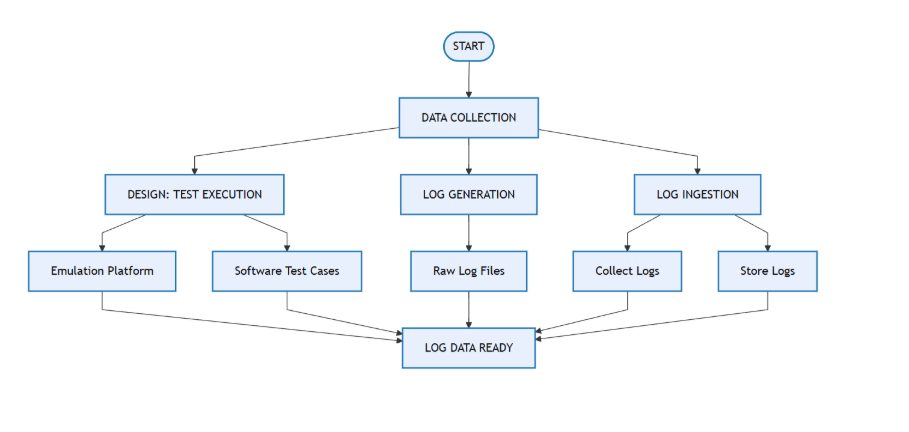
\includegraphics[width=\columnwidth]{Figures/fig1}
\caption{Data collection stage of the proposed pipeline.}
\label{fig:datacoll}
\end{figure}

\subsection{Stage 2 - Log Processing}
The log processing stage takes raw log files as input and produces structured logs and feature vectors. It consists of three parallel paths: a preprocessing path that strips timestamps, ANSI colour codes and platform banner lines; a parsing path that uses LogPAI's Drain algorithm \cite{he2017drain} with a configured similarity threshold and tree depth; and a feature extraction path that builds fixed-length numeric vectors summarizing the activity of each test. The Drain parser walks each token of a log line down a fixed-depth tree, where each leaf corresponds to a unique template; new lines that do not match any existing template at the configured similarity threshold are added as new leaves, allowing the parser to grow incrementally. Figure \ref{fig:logproc} shows the overall log-processing flow.

\begin{figure}[t]
\centering
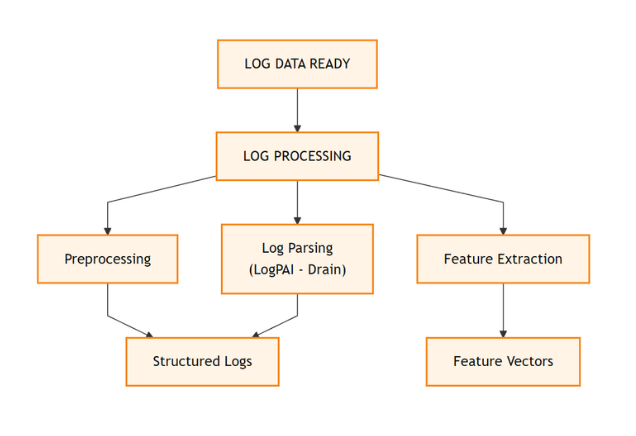
\includegraphics[width=\columnwidth]{Figures/fig2}
\caption{Log processing stage built on LogPAI's Drain algorithm.}
\label{fig:logproc}
\end{figure}

\subsection{Stage 3 - Analysis Engine}
The analysis engine is the core of the pipeline. It consumes the structured logs and feature vectors and is composed of three sub-modules executing in parallel:

\begin{itemize}
\item \textbf{Log Analysis (LogAI):} K-means clustering on the feature vectors groups templates by similarity, and an isolation-forest detector flags anomalous events without the need for hand-labelled training data \cite{cheng2023logai}.
\item \textbf{Metric Extraction:} A curated set of regular expressions, each anchored to its surrounding banner text, extracts deterministic counters such as cycles, IPS, bandwidth, Coproc\_1 and Coproc\_2 work packets, stall counters, scalar activity, spill / fill bytes, and configuration metadata.
\item \textbf{Regression Comparison:} For every (metric, option) pair, the percentage difference against the Cascade baseline is computed using Equation \ref{eq:pctdiff}; degraded tests are flagged using the rule set described in Section III-E.
\item \textbf{LLM Analysis:} For each degraded test, a compact prompt is assembled containing the dominant counters and is sent to an LLM API; the model returns a one-line summary and a directional root-cause hint that becomes part of the per-regression workbook.
\end{itemize}

Figure \ref{fig:analysisengine} captures the internal structure of the analysis engine.

\begin{figure*}[t]
\centering
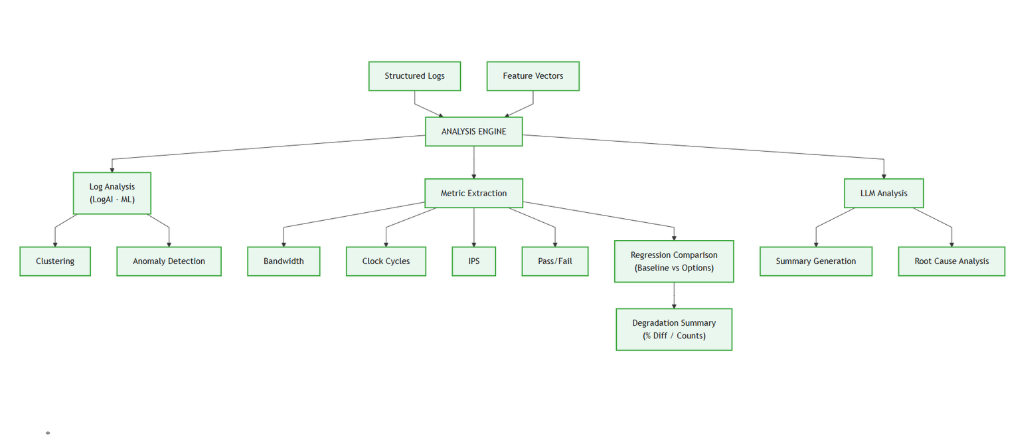
\includegraphics[width=0.95\textwidth]{Figures/fig3}
\caption{Analysis engine, combining LogAI-based ML, regex-driven metric extraction, baseline-vs-options regression comparison and an LLM stage for summary and root-cause direction.}
\label{fig:analysisengine}
\end{figure*}

\subsection{Stage 4 - Output and Delivery}
The output and delivery stage takes the clustering / anomaly results, the degradation summary and the LLM summary and produces two artifacts. The Report Generation path writes a per-regression Excel workbook with three sheets - a \textit{raw} sheet containing every counter extracted from every log, a \textit{derived} sheet containing computed quantities such as percentage differences and ratios, and a \textit{summary} sheet listing only metrics that crossed the degradation threshold - and a multi-option comparison workbook that places the Cascade baseline alongside Nova-Alpha through Nova-Epsilon. The Notification System path posts the workbook link to a project channel and sends a short email digest to the validation lead. Figure \ref{fig:output} illustrates the merge of the three analysis outputs into the two delivery paths.

\begin{figure}[t]
\centering
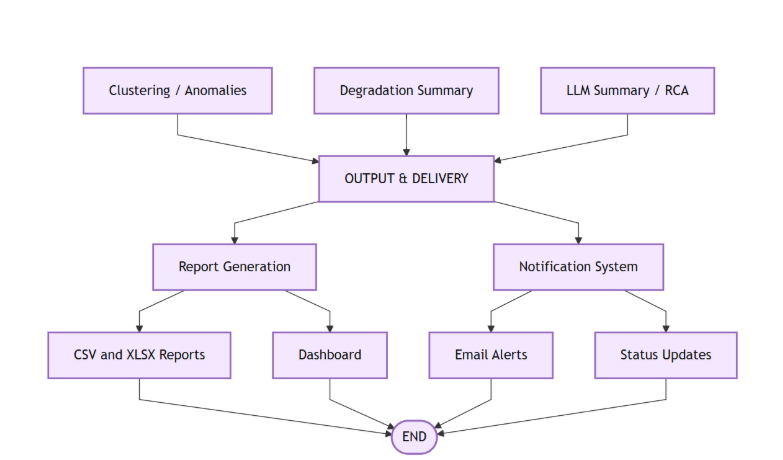
\includegraphics[width=\columnwidth]{Figures/fig4}
\caption{Output and delivery stage producing CSV / XLSX reports, dashboard, email alerts and status updates.}
\label{fig:output}
\end{figure}

\subsection{Computational Formulae}
The percentage difference of a metric \textit{m} on option \textit{o} against the baseline (Cascade) is defined in Equation \ref{eq:pctdiff}.

\begin{equation}
\Delta_{m,o} = \frac{m_o - m_{\text{baseline}}}{m_{\text{baseline}}} \times 100
\label{eq:pctdiff}
\end{equation}

For throughput-style metrics (IPS), a negative $\Delta$ indicates a degradation, whereas for stall and bandwidth-style metrics, a positive $\Delta$ indicates a degradation. A test is flagged as \textit{degraded} when the IPS percentage difference is more negative than a configured threshold (default $-1\%$, chosen tighter than the typical run-to-run variability of $\pm 0.5\%$) \emph{and} at least one stall counter shows a percentage difference larger than ten percent in magnitude.

The clock-frequency speed-up between two options at the same architecture is given by Equation \ref{eq:clock}.

\begin{equation}
S_{f} = \frac{f_{\text{option}}}{f_{\text{baseline}}}
\label{eq:clock}
\end{equation}

This is used to interpret the recovery seen on Nova-Delta and Nova-Epsilon (1037\,MHz) relative to Nova-Alpha (787\,MHz). The expected residual gap, after accounting for clock alone, is given by Equation \ref{eq:residual}.

\begin{equation}
R_{m,o} = \Delta_{m,o} - 100 \cdot \left( S_f - 1 \right)
\label{eq:residual}
\end{equation}

A non-zero $R$ on a throughput metric indicates that the architectural change, and not the clock change, is the dominant cause of the remaining gap; this is the signal that drives root-cause analysis in Section V.

\section{Experimental Setup}

\subsection{Hardware and Software Stack}
The experiments were run inside the in-house emulation environment with the pipeline implemented as follows:
\begin{itemize}
\item \textbf{Operating system:} Linux (Ubuntu / RHEL).
\item \textbf{Language:} Python 3.10.
\item \textbf{Libraries:} Pandas, NumPy and the Python \texttt{re} module for regex; LogPAI for Drain-based parsing; LogAI for clustering and anomaly detection; \texttt{openpyxl} (via Pandas) for multi-sheet Excel workbook generation; an LLM API (GPT / Claude) for summary generation and root-cause hints.
\item \textbf{Source control:} Git.
\item \textbf{Emulation platform:} the Qualcomm emulation platform, which generates the raw log files used by the pipeline.
\end{itemize}

\subsection{Test Suite}
The pipeline is exercised on a fixed test suite of twelve representative graphs spanning vision, language and detection workloads. The graphs are chosen to cover three distinct compute regimes: \textit{Coproc\_1-bound} workloads such as MobileVision and MobileNetV4, \textit{Coproc\_2-bound} workloads such as MobileBERT, MosaicNet, EDSR and the LLaMA prefill graphs, and \textit{DMA-bound} workloads such as the LLaMA decode graphs and VideoDenoise\_HD which stress the memory subsystem and the spill / fill paths. This split ensures that the degradation analysis reaches every part of the silicon under test.

\subsection{Configurations Under Test}
Six configurations are run against this test suite:
\begin{itemize}
\item \textbf{Cascade (787\,MHz):} The reference baseline.
\item \textbf{Nova-Alpha (787\,MHz):} Same clock as Cascade; isolates architectural effects.
\item \textbf{Nova-Beta (787\,MHz):} Second variant at the same clock.
\item \textbf{Nova-Gamma (intermediate):} Used for analysing how clock frequency interacts with architectural changes.
\item \textbf{Nova-Delta (1037\,MHz):} Higher-clock target.
\item \textbf{Nova-Epsilon (1037\,MHz):} Second variant at the higher clock.
\end{itemize}

\subsection{Evaluation Methodology}
The pipeline is validated in three stages. First, on a single \textit{golden} regression where the expected counters are known by hand, the extracted values are compared cell-to-cell against a reference Excel workbook to confirm that every regular expression matches the correct value. Second, on a back-to-back regression where the same option is run twice, the percentage differences are checked to be within the configured noise floor of $\pm 0.5\%$, confirming that the comparison engine does not raise false flags on identical runs. Third, on the full test suite of twelve graphs across six options, the output workbook is reviewed by the validation lead, and the LLM-generated root-cause hints are cross-checked against the underlying counters.

\section{Results and Analysis}

\subsection{Degradation Summary}
Table \ref{tab:degradation} summarizes the number of degraded tests for each configuration on the full test suite of twelve graphs. All regressions passed (zero functional failures); the table reports performance degradations only.

\begin{table}[t]
\caption{Degradation summary across configurations (12 tests each).}
\label{tab:degradation}
\centering
\begin{tabular}{|l|c|c|c|c|}
\hline
\textbf{Option} & \textbf{Tests} & \textbf{Pass} & \textbf{Fail} & \textbf{Degraded}\\
\hline
Cascade (baseline) & 12 & 12 & 0 & --- \\
\hline
Nova-Alpha & 12 & 12 & 0 & 7 \\
\hline
Nova-Beta & 12 & 12 & 0 & 2 \\
\hline
Nova-Gamma & 12 & 12 & 0 & 3 \\
\hline
Nova-Delta & 12 & 12 & 0 & 1 \\
\hline
Nova-Epsilon & 12 & 12 & 0 & 1 \\
\hline
\end{tabular}
\end{table}

The key observations are: (i) Nova-Alpha (running at the same clock frequency as Cascade) shows the most degradations at seven out of twelve, (ii) Nova-Delta and Nova-Epsilon (both 1037\,MHz) show only one degradation each, which is the best result among the Nova variants, (iii) higher clock frequency on the Nova-Delta and Nova-Epsilon configurations compensates for most architectural differences, and (iv) all regressions passed - only performance degradations were observed, not functional failures.

\subsection{Architectural Effect at Same Clock - Nova-Alpha vs.\ Cascade}
To isolate the architectural effect from clock-frequency effects, Figure \ref{fig:ipsdiff} shows the per-graph IPS percentage difference of Nova-Alpha against Cascade, both running at 787\,MHz. Five graphs improve under Nova-Alpha (LLaMA2 prefills and MobileVision variants), while seven graphs degrade. The worst-degraded graph is MosaicNet\_W8A8 at $-24.1\%$ IPS, followed by MobileNetV4\_W8A8 at $-16.4\%$ and MobileDetSSD\_W8A8 at $-11.5\%$. The pattern indicates that the architectural change benefits language-prefill workloads, which are matrix-engine bound, while it hurts vision and detection workloads which are vector-engine bound.

\begin{figure}[t]
\centering
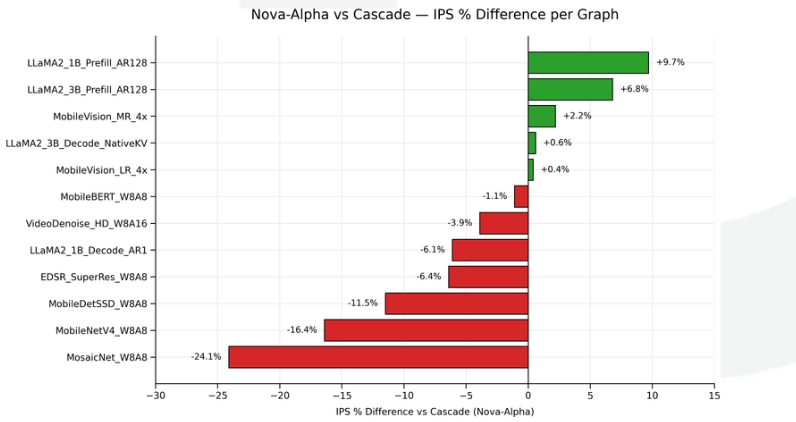
\includegraphics[width=\columnwidth]{Figures/fig5_ipsdiff}
\caption{Nova-Alpha vs.\ Cascade -- IPS percentage difference per graph (same clock).}
\label{fig:ipsdiff}
\end{figure}

\subsection{Root-Cause Analysis: MosaicNet\_W8A8}
MosaicNet\_W8A8 is the worst-degraded test on Nova-Alpha; it is therefore selected as a worked root-cause example. Figure \ref{fig:rca} shows IPS and stall percentage differences across Cascade (787\,MHz), Nova-Alpha (787\,MHz) and Nova-Gamma (1037\,MHz). The IPS values observed are 487.7, 370.4 and 459.5 respectively, corresponding to $-24.1\%$ on Nova-Alpha and $-5.8\%$ on Nova-Gamma relative to Cascade. The Coproc\_2\_STALLS percentage difference is approximately $-113\%$ on both Nova-Alpha and Nova-Gamma, while Coproc\_1\_STALLS percentage difference is around $+54\%$ to $+55\%$ (an improvement) on the Nova variants.

\begin{figure}[t]
\centering
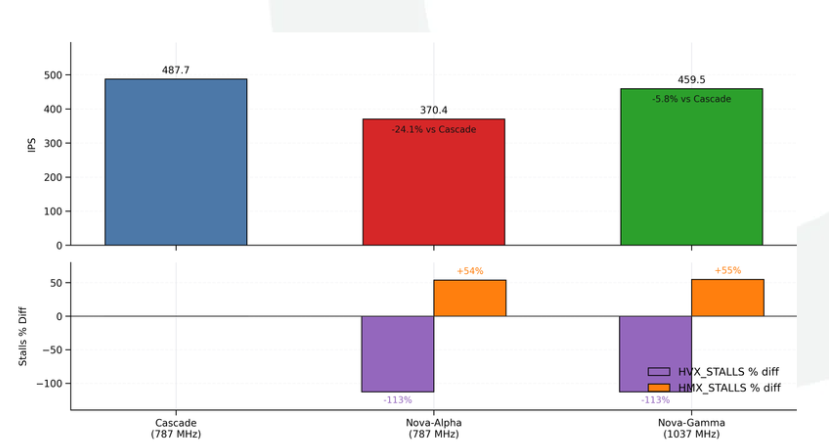
\includegraphics[width=\columnwidth]{Figures/fig6_rca}
\caption{Root-cause analysis of MosaicNet\_W8A8 across Cascade, Nova-Alpha and Nova-Gamma. Top: IPS bars. Bottom: Coproc\_1 and Coproc\_2 stalls percentage difference relative to baseline.}
\label{fig:rca}
\end{figure}

The interpretation, supported by Equations \ref{eq:pctdiff}--\ref{eq:residual}, is as follows:
\begin{itemize}
\item At 787\,MHz (Nova-Alpha), Coproc\_2 stalls explode ($-113\%$): the vector engine is severely starved.
\item At 1037\,MHz (Nova-Gamma), Coproc\_2 stalls remain similar in absolute terms but the higher clock compensates, and the IPS gap recovers from $-24.1\%$ to $-5.8\%$.
\item Coproc\_1 stalls actually improve on the Nova variants (fewer matrix-engine stall cycles), confirming that the matrix engine is not the bottleneck on this graph.
\item The remaining $-5.8\%$ at 1037\,MHz is due to Coproc\_2 stalls that the higher clock cannot fully compensate; this is the residual architectural gap $R$ defined in Equation \ref{eq:residual} and points engineers towards the Coproc\_2 scheduling path as the next investigation step.
\end{itemize}

The LLM-generated summary for this test correctly identified \textit{Coproc\_2 starvation due to insufficient vector-engine scheduling on the Nova architecture} as the most likely cause, matching the conclusion drawn from the manual analysis.

\subsection{Wall-Clock Time Comparison}
A direct wall-clock comparison was carried out between the manual workflow and the proposed pipeline on the same six-option, twelve-graph regression. The manual workflow took between approximately 90 and 180 minutes per regression, with most of the time spent on grepping, transcription and spreadsheet formatting rather than on technical analysis. The proposed pipeline completed the same regression in approximately two minutes on the standard development server, a speed-up of roughly $50\times$ to $90\times$. Crucially, the pipeline output is deterministic and bit-exactly reproducible by any other engineer, which the manual workflow was not.

\subsection{Comparison with Baseline Approaches}
A simple baseline that uses only regex-based extraction without any clustering or LLM stage matches the metric extraction quality of the proposed pipeline but cannot produce summaries or root-cause hints for degraded tests. A second baseline that uses LogAI alone for unsupervised anomaly detection produces useful clusters of anomalous events but does not surface the targeted comparison-against-baseline metrics expected by the validation team. The proposed hybrid pipeline subsumes both baselines and additionally adds the LLM-based summarization and root-cause direction stage, which is the most heavily used part of the output by validation engineers in practice.

\section{Discussion}

\subsection{Technical Contributions}
The proposed pipeline demonstrates that a hybrid integration of deterministic parsers (Drain), classical machine learning (LogAI), and Large Language Models can be combined under a single execution context to address an industrial validation problem. The decision to keep deterministic regex-based extraction at the heart of the metric extraction stage, while delegating only summary generation and root-cause direction to the LLM, is deliberate: it ensures that the numerical content of every regression report is verifiable and reproducible, while still gaining the productivity benefit of natural-language summaries.

The combined degradation rule that requires both an IPS gap and a stall-counter spike is a small but practically important contribution: it suppresses the false-positive rate that a naive IPS-only threshold would suffer from, particularly on graphs where run-to-run variance is close to the configured threshold.

\subsection{Practical Implications}
\subsubsection{Industrial Workflow}
The two-minute regression turn-around enables the validation team to evaluate many more silicon configurations within the same time budget, which directly accelerates pre-silicon performance bring-up.

\subsubsection{Cross-Engineer Reproducibility}
Standardized three-sheet workbooks remove inter-engineer variability in counter naming and aggregation. Two engineers running the pipeline on the same regression now produce bit-exactly identical outputs.

\subsubsection{Integration with Build Systems}
The deterministic, scriptable nature of the pipeline allows it to be integrated as a continuous regression service, posting workbook links and email digests automatically when builds finish.

\subsection{Limitations and Challenges}
\subsubsection{Confidentiality of Log Formats}
The Drain templates and the regex set are tuned to the in-house log format of the emulation platform. Cross-vendor portability would require either a re-tuning of these patterns or the adoption of LLM-based parsers such as those proposed in \cite{le2023logprompt, zhang2025semanticlog}.

\subsubsection{Advisory Nature of LLM Hints}
The LLM-generated root-cause hints are advisory only. Final engineering decisions are still taken by validation engineers after reviewing the structured workbooks. Further work is needed to quantify the accuracy of these hints across a broader corpus of regressions.

\subsubsection{Test Suite Scope}
The reported results are based on a fixed test suite of twelve graphs and six configurations. Generalization to larger suites and to other silicon programs has not yet been formally evaluated.

\subsection{Future Research Directions}
\subsubsection{Semantic Parsing}
Replacing the curated regex set with a semantic, LLM-driven parser \cite{le2023logprompt, zhang2025semanticlog} would allow the pipeline to ingest logs from multiple emulation and silicon platforms without manual tuning.

\subsubsection{Supervised Anomaly Detection}
Extending the LogAI module with supervised anomaly detection trained on labelled regressions would let the system rank degradations by likelihood of being functional rather than purely architectural.

\subsubsection{Continuous Regression Mode}
Running the pipeline as a long-lived service that posts results to a dashboard in real time, instead of being invoked per regression, would close the loop between build completion and engineering attention.

\subsubsection{Build-System Coupling}
Correlating detected root causes - compiler version, build flags, hardware register settings - with code changes in the build system would enable the pipeline to suggest the specific commit responsible for a regression, going beyond directional root-cause hints.

\section{Conclusion}

This paper has presented an AI-based automated log analysis and performance evaluation system for emulation-based pre-silicon software testing. The proposed pipeline integrates LogPAI's Drain algorithm for structured parsing, LogAI for unsupervised clustering and anomaly detection, regex-driven extraction for deterministic counters, and an LLM API for natural-language summary and root-cause direction. Implemented in Python 3 on a Linux-based emulation environment, the pipeline replaces the slow and error-prone manual workflow used by the pre-silicon performance validation team with a single, reproducible execution that completes a full regression analysis in approximately two minutes.

\subsection{Key Achievements}
\begin{itemize}
\item \textbf{Hybrid pipeline:} A four-stage pipeline that combines deterministic parsers, classical machine learning and LLM-based reasoning under a single execution context.
\item \textbf{Quantitative validation:} On a fixed test suite of twelve graphs and six configurations, the pipeline correctly ranks Nova-Alpha (787\,MHz) as the worst with seven degraded tests and Nova-Delta / Nova-Epsilon (1037\,MHz) as the best with one degradation each.
\item \textbf{Productivity gains:} A reduction of regression analysis time from approximately 90--180 minutes of manual work to about 2 minutes of pipeline execution, with deterministic and reproducible outputs.
\item \textbf{Worked root-cause example:} A detailed analysis of MosaicNet\_W8A8 isolates Coproc\_2 stalls as the dominant bottleneck, with the IPS gap shrinking from $-24.1\%$ at 787\,MHz to $-5.8\%$ at 1037\,MHz, supported by Equations \ref{eq:pctdiff}--\ref{eq:residual}.
\end{itemize}

\subsection{Research Impact}
The work contributes to the broader field of log-based performance regression analysis by demonstrating the practical viability of a hybrid AI pipeline in an industrial pre-silicon validation flow. It provides a reference implementation, a degradation-flagging rule set, and a worked root-cause analysis methodology that other validation teams can adapt to their own emulation environments.

\subsection{Future Outlook}
The continued growth of emulation-based validation, combined with the rapid maturation of LLM-based code understanding and log analysis, points to several promising directions: semantic parsing for cross-platform portability, supervised anomaly detection for ranked degradation lists, real-time dashboards driven by long-lived pipeline services, and tighter coupling with the build system so that root causes can be traced back to specific commits. The pipeline presented here is a step in that direction.

\subsection{Closing Remarks}
As pre-silicon validation continues to consume an ever-larger share of the SoC development cycle, automated and reproducible analysis pipelines become an essential productivity tool rather than a convenience. The combination of deterministic parsing, classical machine learning and Large Language Models, demonstrated in this work, offers a practical pathway to industrial-scale log analysis with both quantitative rigor and natural-language interpretability.

\section*{Acknowledgments}
The authors gratefully acknowledge the support of RV College of Engineering, Bangalore, and Qualcomm India Pvt.\ Ltd.\ for providing the resources, infrastructure, and mentorship that made this work possible. Special thanks to Dr.\ Roopa J of the Department of Electronics and Communication Engineering, RV College of Engineering, for her academic guidance, and to Mr.\ Venkatarakesh Mamidi, Senior Staff Engineer at Qualcomm India Pvt.\ Ltd., for his continuous technical mentorship throughout the internship.

\begin{thebibliography}{99}

\bibitem{he2017drain}
P. He, J. Zhu, Z. Zheng, and M. R. Lyu, ``Drain: An online log parsing approach with fixed depth tree,'' in \textit{IEEE International Conference on Web Services (ICWS)}, 2017, pp. 33--40.

\bibitem{zhu2019tools}
J. Zhu, S. He, J. Liu, P. He, Q. Xie, Z. Zheng, and M. R. Lyu, ``Tools and benchmarks for automated log parsing,'' in \textit{IEEE/ACM International Conference on Software Engineering: Software Engineering in Practice (ICSE-SEIP)}, 2019, pp. 121--130.

\bibitem{du2016spell}
M. Du and F. Li, ``Spell: Streaming parsing of system event logs,'' in \textit{IEEE International Conference on Data Mining (ICDM)}, 2016, pp. 859--864.

\bibitem{du2017deeplog}
M. Du, F. Li, G. Zheng, and V. Srikumar, ``DeepLog: Anomaly detection and diagnosis from system logs through deep learning,'' in \textit{ACM Conference on Computer and Communications Security (CCS)}, 2017, pp. 1285--1298.

\bibitem{zhang2019logrobust}
X. Zhang, Y. Xu, Q. Lin, B. Qiao, H. Zhang, Y. Dang, C. Xie, X. Yang, Q. Cheng, Z. Li, J. Chen, X. He, R. Yao, J.-G. Lou, M. Chintalapati, F. Shen, and D. Zhang, ``Robust log-based anomaly detection on unstable log data,'' in \textit{ACM Joint Meeting on European Software Engineering Conference and Symposium on the Foundations of Software Engineering (ESEC/FSE)}, 2019, pp. 807--817.

\bibitem{guo2021logbert}
H. Guo, S. Yuan, and X. Wu, ``LogBERT: Log anomaly detection via BERT,'' in \textit{International Joint Conference on Neural Networks (IJCNN)}, 2021, pp. 1--8.

\bibitem{cheng2023logai}
Q. Cheng, A. Saha, W. Yang, C. Liu, D. Sahoo, and S. Hoi, ``LogAI: A library for log analytics and intelligence,'' arXiv preprint arXiv:2301.13415, 2023.

\bibitem{he2021survey}
S. He, P. He, Z. Chen, T. Yang, Y. Su, and M. R. Lyu, ``A survey on automated log analysis for reliability engineering,'' \textit{ACM Computing Surveys}, vol. 54, no. 6, pp. 1--37, 2021.

\bibitem{lai2018emulation}
G. Lai and W. Kuo, ``Emulation-based pre-silicon system performance verification,'' \textit{IEEE Design \& Test}, vol. 35, no. 6, pp. 7--14, 2018.

\bibitem{deltombe2014emulation}
S. Deltombe, ``Hardware emulation in pre-silicon system performance validation,'' in \textit{Design and Verification Conference and Exhibition (DVCon)}, 2014.

\bibitem{le2023logprompt}
V.-H. Le and H. Zhang, ``Log parsing with prompt-based few-shot learning,'' in \textit{IEEE/ACM International Conference on Software Engineering (ICSE)}, 2023, pp. 2438--2449.

\bibitem{liu2024logprompt}
Y. Liu, S. Tao, W. Meng, J. Wang, W. Ma, Y. Chen, Y. Zhao, H. Yang, and Y. Jiang, ``LogPrompt: Prompt engineering towards zero-shot and interpretable log analysis,'' in \textit{IEEE/ACM International Conference on Software Engineering: Companion Proceedings (ICSE-Companion)}, 2024, pp. 364--365.

\bibitem{ahmed2023recommending}
T. Ahmed, S. Ghosh, C. Bansal, T. Zimmermann, X. Zhang, and S. Rajmohan, ``Recommending root-cause and mitigation steps for cloud incidents using large language models,'' in \textit{IEEE/ACM International Conference on Software Engineering (ICSE)}, 2023, pp. 1737--1749.

\bibitem{vaswani2017attention}
A. Vaswani, N. Shazeer, N. Parmar, J. Uszkoreit, L. Jones, A. N. Gomez, L. Kaiser, and I. Polosukhin, ``Attention is all you need,'' in \textit{Advances in Neural Information Processing Systems (NeurIPS)}, 2017, pp. 5998--6008.

\bibitem{brown2020gpt3}
T. B. Brown \textit{et al.}, ``Language models are few-shot learners,'' in \textit{Advances in Neural Information Processing Systems (NeurIPS)}, 2020, pp. 1877--1901.

\bibitem{zhang2025semanticlog}
Y. Zhang \textit{et al.}, ``SemanticLog: Towards effective and efficient large-scale semantic log parsing,'' \textit{IEEE}, 2025.

\bibitem{liu2025luk}
X. Liu \textit{et al.}, ``LUK: Empowering log understanding with expert knowledge from large language models,'' \textit{IEEE Transactions on Software Engineering}, 2025.

\bibitem{wang2025logdlr}
H. Wang \textit{et al.}, ``LogDLR: Unsupervised cross-system log anomaly detection through domain-invariant latent representation,'' \textit{IEEE}, 2025.

\bibitem{chen2025epas}
Z. Chen \textit{et al.}, ``EPAS: Efficient online log parsing via asynchronous scheduling,'' in \textit{IEEE International Conference on Data Engineering (ICDE)}, 2025.

\bibitem{li2025practitioners}
J. Li \textit{et al.}, ``Practitioners' expectations on log anomaly detection,'' \textit{IEEE Transactions on Software Engineering}, 2025.

\end{thebibliography}

\end{document}
